\documentclass[tikz]{standalone}

\begin{document}
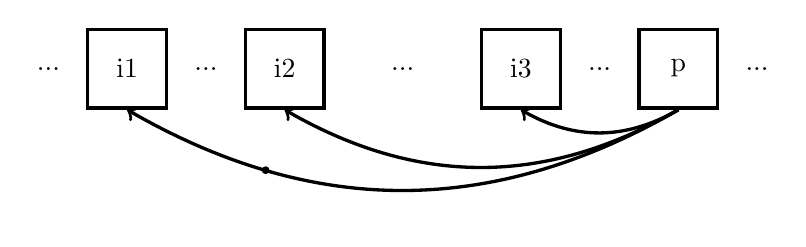
\begin{tikzpicture}[
    very thick,
    mignode/.style={
        rectangle,
        draw,
        inner sep=0pt,
        minimum size=1cm,
    },
]

    \node at (0,0) {...};
    \node[mignode] (ch1) at (1,0) {i1};
    \node at (2,0) {...};
    \node[mignode] (ch2) at (3,0) {i2};
    \node at (4.5,0) {...};
    \node[mignode] (ch3) at (6,0) {i3};
    \node at (7,0) {...};
    \node[mignode] (p)   at (8,0) {p};
    \node at (9,0) {...};

    \draw[->] (p.south) to[bend left] (ch3.south);
    \draw[->] (p.south) to[bend left] (ch2.south);
    \draw[->] (p.south) to[bend left] node[circle,fill,inner sep=1pt,near end]{}(ch1.south);

\end{tikzpicture}
\end{document}